\documentclass{article}

    \usepackage{xcolor}
    \definecolor{pf}{rgb}{0.4,0.6,0.4}
    \usepackage[top=1in,bottom=1in, left=0.8in, right=0.8in]{geometry}
    \usepackage{setspace}
    \setstretch{1.2} 
    \setlength{\parindent}{2em}

    \usepackage{paralist}
    \usepackage{cancel}

    % \usepackage{ctex}
    \usepackage{amssymb}
    \usepackage{amsmath}
    
    \usepackage{extarrows}
    \usepackage{tikz-cd}
    \usetikzlibrary{arrows}

    \usepackage{float}

    \usepackage{tcolorbox}
    \definecolor{Df}{RGB}{0, 184, 148}
    \definecolor{Th}{RGB}{9, 132, 227}
    \definecolor{Rmk}{RGB}{215, 215, 219}
    \newtcolorbox{Df}[2][]{colbacktitle=Df, colback=white, title={\large\color{white}#2},fonttitle=\bfseries,#1}
    \newtcolorbox{Th}[2][]{colbacktitle=Th, colback=white, title={\large\color{white}#2},fonttitle=\bfseries,#1}
    \newtcolorbox{Rmk}[2][]{colbacktitle=Rmk, colback=white, title={\large\color{black}{Remarks}},fonttitle=\bfseries,#1}

    \title{\LARGE \textbf{Geometrical Rigorous Definition of Trigonometric Functions}}
    \author{\large Jiawei Hu}
    
    % new commands for formula typying
    \newcommand{\parfrac}[2]{\frac{\partial #1}{\partial #2}}
    \newcommand{\biparfrac}[2]{\frac{\partial^2 #1}{#2}}
    \newcommand{\dif}{\mathop{}\!\mathrm{d}}
    \newcommand{\Dif}{\mathop{}\!\mathrm{D}}
\begin{document}

\maketitle
\tableofcontents
\newpage

This is a problem file about the \textbf{geometrical rigorous definition of trigonometric functions}.  

By the way, we now reiterate some commonly-used notations and conventions:
\begin{compactenum}
    \item $\mathbb{R}$: the set of the real numbers;
    \item $\mathbb{R}^+$: the set of the positive real numbers;
    \item $\mathbb{N}$: the set of the natural numbers;
    \item $\mathbb{N^\ast}$ or $\mathbb{N}^+$: the set of the positive integers.
    \item An agreement for the length of a list: if we write $a_1, \dots, a_n$, then we indicate that $n$ is finite and that $n\geq 1$; if we write $a_0, \dots, a_n$, then we indicate that $n$ is finite and that $n\geq 0$.
    \item This text involves inner product and norm in $\mathbb{R}^n$, which refers to the most common ones — the norm is the $L2$-norm.
\end{compactenum} 
Please check the notations and definitions by yourself from the previous chapters or courses. Then with everything prepared, here we go.

\noindent\rule{\textwidth}{2pt}

\section{Introduction}
Although the trigonometric functions $\sin x$ and $\cos x$ are already well studied early during a student's high school years, and are at that time defined by the unit circle (which is very intuitive and elegant), this definition is still not rigorous, as it is based on the geometric intuition of the \textbf{arc length}. Since we are already exposed to the language of inner product space (for length, angle, etc.) and calculus (for curve, limit, etc.), it's time to give a rigorous definition of the trigonometric functions, combining the geometric intuition and the rigorous calculus.

Hence, if you have already felt comfortable with the previous definition of $\sin x$ and $\cos x$, you can just skip this text. After all, rigorousness is not the only thing that matters in mathematics. 

\section{Preliminaries: parametric curves, tangent vectors, and arc length}
Different subsets of points in $\mathbb{R}^n$ vary a lot, and proper parametrization characterizes the properties of a given subset. 

\begin{Df}{Df 10\_P1.4.1 (parametric curve)}
    A \textbf{parametric curve} (or \textbf{parametrized curve}) in $\mathbb{R}^n$ is a $1$-real $n$-function $\pmb{x}$ defined on an interval $I\subset \mathbb{R}$. The image of the curve $\pmb{x}$ is called the \textbf{trace} of the curve.
\end{Df}

Unlike the statement in Df \{, ID: 7.7\}, here a curve does not refers to the subset of $\mathbb{R}^n$ itself, but the \textbf{parameter equations} 
$$ \pmb{x}(t) = (x_1(t), \dots, x_n(t)), \quad t\in I. $$
This does not conflict with Df \{, ID: 7.7\}, it is a just an abstraction instead. With this definition, a parametrized curve $\pmb{x}: I\rightarrow \mathbb{R}^n$ is called $\mathcal{C}^1$ if $\pmb{x}\in \mathcal{C}^1(I)$; and a $\mathcal{C}^1$ curve is called \textbf{regular} or \textbf{smooth} if $\pmb{x}'(t)\neq \pmb{0}$ for all $t\in I$. This is just what Df \{, ID: 7.7\} said.

The most common curves we know, say, in a piece of paper $\mathbb{R}^2$, are those able to be drawn by a pen without lifting it from the paper. \textcolor{Df}{These curves are discribed as \textbf{continuous curves} or $\mathcal{C}^{0}$ curves ($\mathcal{C}^0$ means $\pmb{x}\in \mathcal{C}^0(I)$ of course)}. Now imagine that your finger touches and moves along the curve, and in this process no sudden change of direction occurs. This is what ``smooth'' literally means, and it is rational to desicribe it by $\mathcal{C}^1$. 

For a $\mathcal{C}^1$ curve $\pmb{x}(t)$, a particle moves along the curve as the time $t$ varies. How to compute the velocity of the particle at a moment $t_0$? Naturally, it is
$$ \pmb{v}(t_0) \triangleq \lim_{t\rightarrow t_0} \frac{\pmb{x}(t) - \pmb{x}(t_0)}{t-t_0} = \pmb{x}'(t_0) = (\pmb{x}_1'(t_0), \cdots, \pmb{x}_n'(t_0)). $$
This is just the \textbf{tangent vector}.

\begin{Df}{Df 10\_P1.4.2 (tangent vector)}
    For a $\mathcal{C}^1$ curve $\pmb{x}: I\rightarrow \mathbb{R}^n$, the \textbf{tangent vector} at a point $t_0\in I$ is the vector $\pmb{x}'(t_0)$.
\end{Df}

Hence, the parameter equation $\pmb{x}(t)$ specifies anything of the motion of a particle during some time interval $t\in I$. The particle may move along the curve in the velocity $\pmb{v}(t) = \pmb{x}'(t)$, but it may also move in another. Therefore we define an equivalence relation to remove this difference:

\begin{Df}{Df 10\_P1.4.2.1 (equivalent parametrized curves)}
    Two parametrized curves $t\mapsto \pmb{x}(t)$ ($t\in I$) and $\tilde{t}\mapsto \tilde{\pmb{x}}(\tilde{t})$ ($\tilde{t}\in \tilde{I}$) are said to be \textbf{equivalent} if 
    $$ \pmb{x}(t) = \tilde{\pmb{x}}(\tilde{t}) $$
    for some $\mathcal{C}^1$ bijection $t\mapsto \tilde{t}$ (from $I$ to $\tilde{I}$) such that
    $$ \frac{\dif\tilde{t}}{\dif t} > 0. $$
\end{Df}

\textcolor{Th}{This is exactly an equivalence relation.} Then for two equivalent parametrized curves $\pmb{x}(t)$ and $\tilde{\pmb{x}}(\tilde{t})$, the velocities of the particle at some moment $t_0$ share the same orientation, and differ only in the magnitude:

\begin{Th}{Th 10\_P1.4.2.2}
    Suppose $\pmb{x}(t)$ and $\tilde{\pmb{x}}(\tilde{t})$ are equivalent parametrized curves. Then for any $t_0$,
    $$ \pmb{x}'(t_0) = c\, \tilde{\pmb{x}}'(\tilde{t}_0) $$
    for some $c>0$.
    \tcblower
    \textit{Pf}: Use the chain rule.
\end{Th}

This theorem mathematically justifies the possibility of adjusting the speed of the particle, and lead us to the uniform-speed parametrization that $\|\pmb{x}'(t)\|$ is a constant, especially, $1$. Not only would we like to show the existence of such a parametrization, but also we would clarify that the parametrization here is \textbf{arc-length-parametrized}.

Before going ahead, we clarify that the equivalence relation just defined is authentic, that is, \textcolor{Th}{whether a parametric curve is
\begin{compactenum}
    \item continuous
    \item $\mathcal{C}^1$
    \item smooth
    \item piecewise-smooth
    \item closed
    \item simple
\end{compactenum}
or not, is independent of which equivalent parametrization is chosen.} In other word, if a parametric curve $\pmb{x}$ is continuous (resp. $\mathcal{C}^1$) (resp. smooth) (resp. piecewise-smooth) (resp. closed) (resp. simple), then so is any $\tilde{\pmb{x}}$ equivalent to $\pmb{x}$. Also, \textcolor{Th}{the path length (the Df \{, ID: 7.7.1\}) of a $\mathcal{C}^1$ curve (or a piecewise-smooth curve) is independent of which equivalent parametrization is chosen}.

\begin{Th}{Th 10\_P1.4.3 (parametrized by arc length)}
    \textcolor{Th}{For a regular curve $\pmb{x}(t)$, the arc length $s(t_0, t)$ measured from $t_0$ to $t$ can be defined (known early in Th \{, ID: 7.7.1\}):
    $$ s(t_0, t) = \int_{t_0}^t \|\pmb{x}'(\tau)\|\dif \tau \triangleq s(t). $$}
    Then:
    \begin{compactenum}
        \item $t\mapsto s(t)$ is a $\mathcal{C}^1$, strictly increasing function. And thus:
        \item The curve $\pmb{x}(t)$ can be equivalently reparametrized by $s$:
        $$ \pmb{x}(t) = \tilde{\pmb{x}}(s). $$
        \item The reparametrization $\tilde{\pmb{x}}(s)$ yields $\|\tilde{\pmb{x}}'(s)\| = 1$.
        \item If conversely $\pmb{x}(t)$ has already satisfied $\|\pmb{x}'(t)\| = 1$, then
        $$ s = \int_{t_0}^t \dif \tau = t - t_0, $$
        i.e., $t$ is the arc length measured from some other point.
    \end{compactenum}
    \tcblower
    \textit{Pf}: 
    \begin{compactenum}
        \item Differentiate $s$ w.r.t. $t$:
        $$ \frac{\dif s}{\dif t} = \frac{\dif}{\dif t} \int_{t_0}^t \|\pmb{x}'(\tau)\|\dif \tau = \|\pmb{x}'(t)\| > 0. $$
        \item Obvious;
        \item Use the chain rule;
        \item Obvious.
    \end{compactenum}
\end{Th}

\textcolor{Th}{By the way, the $\pmb{x}(t)$ in this theorem is not necessary to be regular (to holds $\pmb{x}^\prime (t) \neq 0$) for the reparametrization by $s$. Actually, the $\mathcal{C}^1$ curve $\pmb{x}(t)$ only needs to make sure that $s(t)$ is strictly increasing (e.g. $\|\pmb{x}^\prime (t)\| = 0$ for only a finite number of $t$, or other cases in Th \{, ID: 3.6.1.1\}), and then the reparametrization by $s$ is still valid.}

\section{Definition of $\sin \theta$ and $\cos \theta$}
Now apply the above results to found the rigorous definition of $\sin \theta$ and $\cos \theta$. Consider the unit circle
$$ C = \{ (x, y)\in \mathbb{R}^2: x^2 + y^2 = 1 \}. $$
An explicit parametrization, say, $(x, f(x))$ is needed to start with. Since the circle is multi-valued for almost all $x$ (resp. $y$), we need to split $C$ into four quadrants:
$$
\begin{aligned}
    & C_1 = \{ (x, y)\in C: x\geq 0, y\geq 0 \} \qquad A_1 = (1, 0),\, B_1 = (0, 1) \\
    & C_2 = \{ (x, y)\in C: x\leq 0, y\geq 0 \} \qquad A_2 = (0, 1),\, B_2 = (-1, 0) \\
    & C_3 = \{ (x, y)\in C: x\leq 0, y\leq 0 \} \qquad A_3 = (-1, 0),\, B_3 = (0, -1) \\
    & C_4 = \{ (x, y)\in C: x\geq 0, y\leq 0 \} \qquad A_4 = (0, -1),\, B_4 = (1, 0)
\end{aligned}
$$
and we can first deal with $C_1$, and then inductively extend all work to others. 

\subsection{Trigonometric Function within $C_1$}
For $C_1$, we first have the explicit parametrization:
$$ C_1: 
\begin{cases}
    x(t) = \sqrt{1-t^2} \\
    y(t) = t
\end{cases} \qquad (t\in [0, 1])
$$
Hence it is $\mathcal{C}^1$ for $t\in [0,1)$, with the arc length $\theta$ measured from $0$ to $t$:
$$ \theta = \theta (t) = \int_0^t \sqrt{(x^\prime (\tau))^2 + (y^\prime (\tau))^2}\dif \tau = \int_0^t \frac{1}{\sqrt{1-\tau^2}}\dif \tau $$ 
for every $t\in [0, 1)$. \textcolor{Th}{Since $\theta(1)$ is an improper integral with improper point $1$, we need to check its convergence:}
$$ \textcolor{Df}{\frac{\pi}{2} \triangleq } \;\textcolor{Th}{\theta(1) = \int_0^1 \frac{1}{\sqrt{1-\tau^2}}\dif \tau \leq \int_0^1 \frac{1}{\sqrt{1-\tau}}\dif \tau = 2.} $$
\textcolor{Th}{And then $t\mapsto \theta(t)$ is strictly increasing (on $t\in [0, 1]$), and is $\mathcal{C}^1$ on $(0, 1)$}. Hence $(x(t), y(t))$ can be reparametrized by $\theta$:
$$ C_1:
\begin{cases}
    x(\theta) \; \textcolor{Df}{\triangleq \cos \theta} \\
    y(\theta) \; \textcolor{Df}{\triangleq \sin \theta}
\end{cases} \qquad (\theta\in [0, \frac{\pi}{2}])
$$
and we have known that \textcolor{Th}{as $\theta$ varies from $0$ to $\pi/2$, $\cos \theta$ continuously decreases from $1$ to $0$, and $\sin \theta$ continuously increases from $0$ to $1$.}

\subsection{Extended Trigonometric Function within $C_2$}
The extension is based on the symmetry of the circle under the rotation $P_{\pi/2}$:
$$ P_{\pi/2}: (x, y)\mapsto (-y, x), $$ 
which is a linear isometry on the inner product space $\mathbb{R}^2$. Clearly, the circle $C$ satisfies:
$$ P_{\pi/2} (C_1) = C_2, $$
and more generally:
$$ P_{\pi/2} (C_k) = C_{k+1}, \qquad \forall k\in\mathbb{Z} $$ 
by which we define the $C_k$ for all $k\in\mathbb{Z}$. With this symmetry of rotation, we can just simply copy all the work in $C_1$ to $C_2$, via the isomorphism $P_{\pi/2}$:

% $$
% \begin{tikzcd}
%     A \arrow[cm double to - cm left hook]{r} & B \\
%     C_1 \arrow[hook, two heads]{r}{P_{\pi/2}} & C_2
% \end{tikzcd}
% $$

\begin{figure}[H]
    \centering
    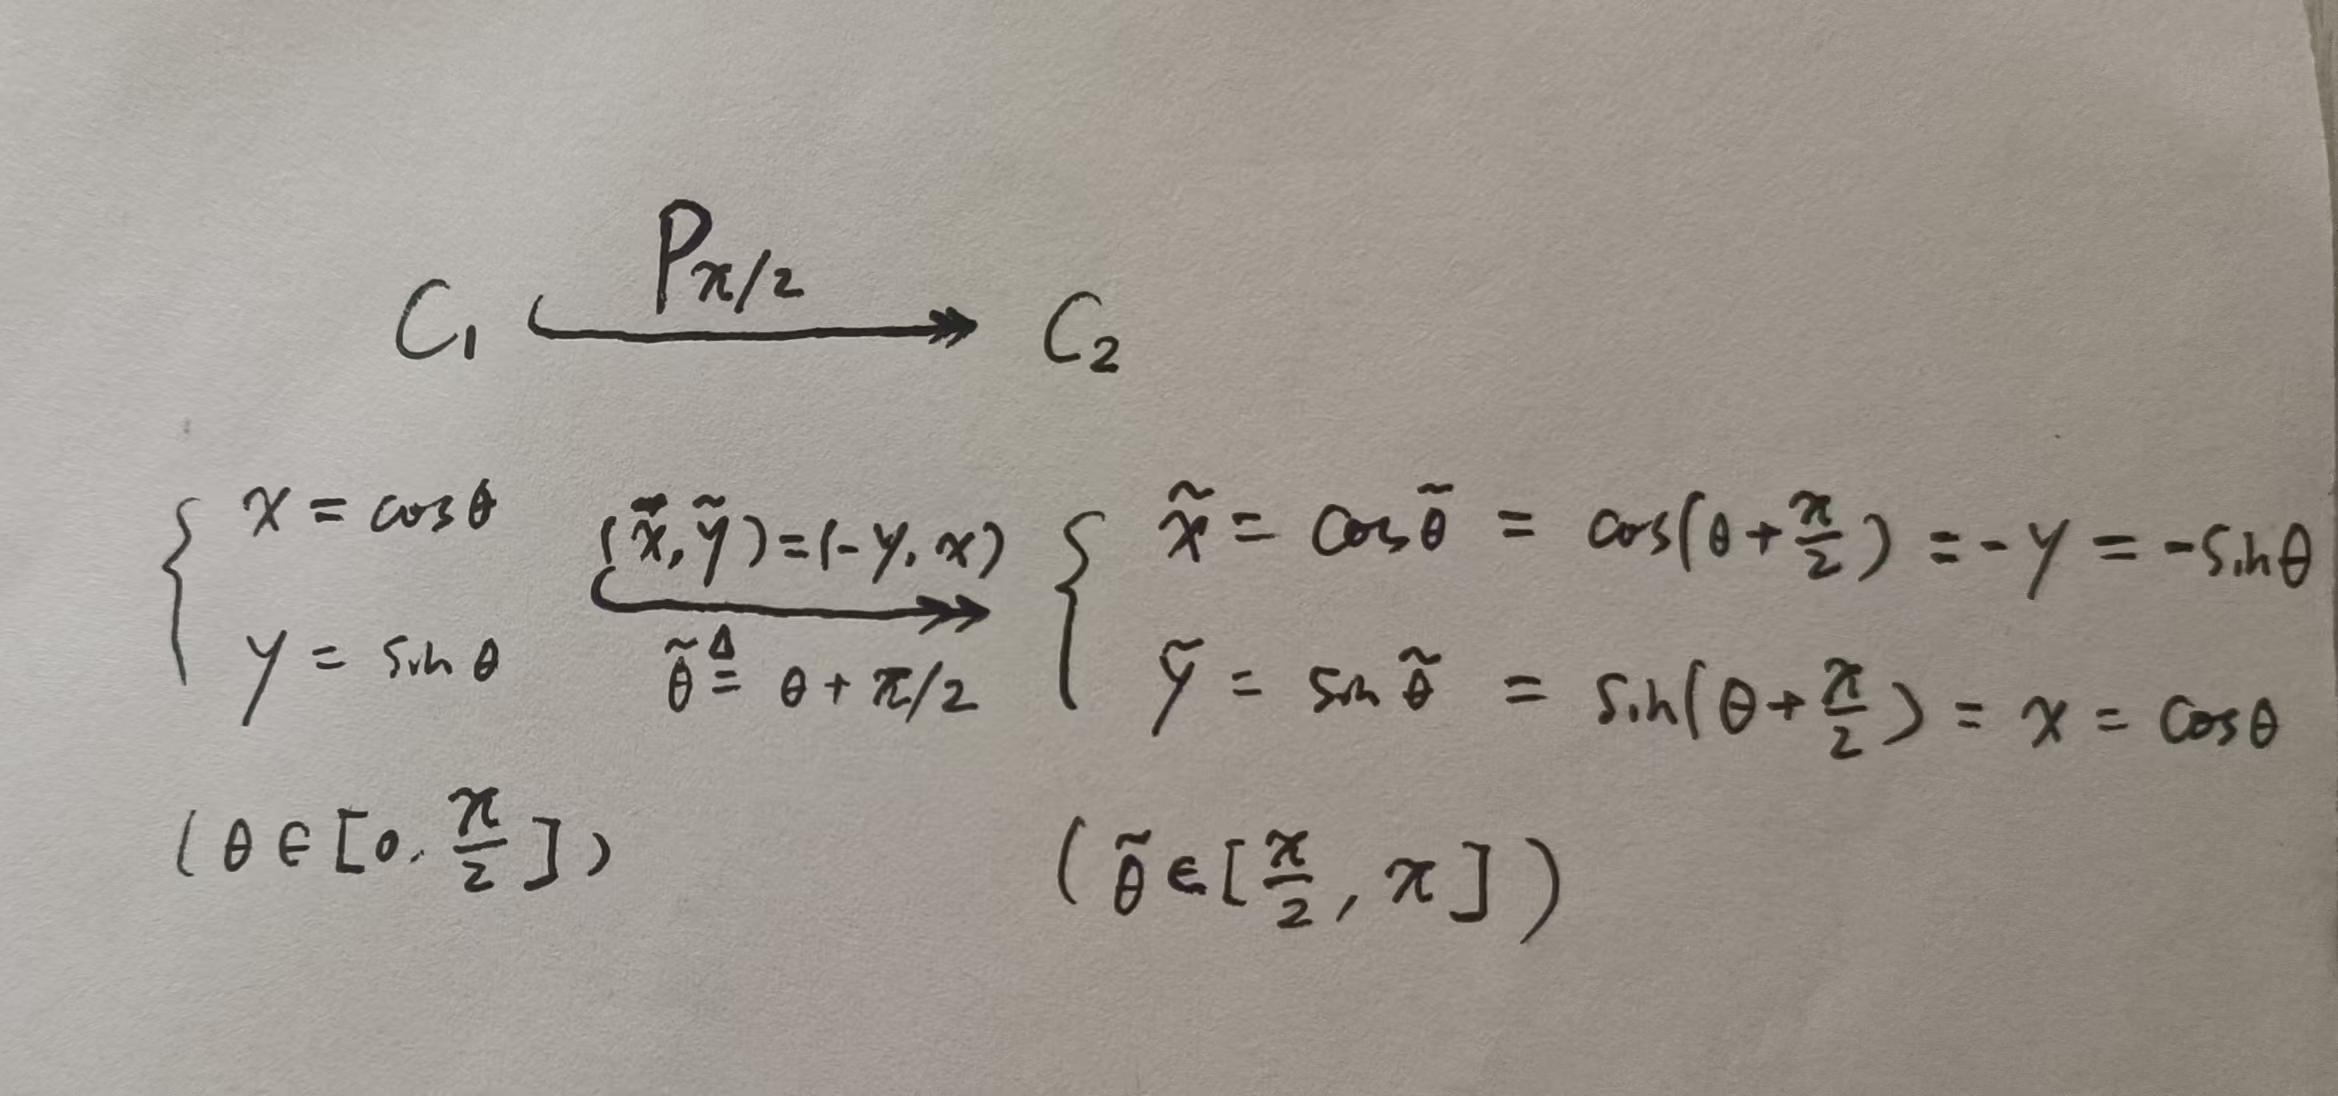
\includegraphics[width=0.7\textwidth]{figs_P1/1.jpg}
    \caption{Copying the work in $C_1$ to $C_2$}
    \label{fig:c1_to_c2}
\end{figure}

Here the hook-arrow $\hookrightarrow$ means the correspondence is injective, and the two-head-arrow $\twoheadrightarrow$ means the correspondence is surjective. In the figure we write 
\begin{tikzcd}
    C_1 \arrow[hook, two heads]{r}{P_{\pi/2}} & C_2
\end{tikzcd}
to indicate that the correspondence $P_{\pi/2}$ is both injective and surjective, i.e. is bijective. While copying the work in $C_1$ to $C_2$, we reparametrize $C_2$ by $\tilde{\theta} \in [\pi/2, \pi]$ rather than $\theta \in [0, \pi/2]$, and set $\tilde{\theta} = \theta + \pi/2$. Hence we immediately obtain the induction formulae for $\cos \theta$ and $\sin \theta$, which express $\cos (\theta + \pi/2)$ (resp. $\sin (\theta + \pi/2)$) in terms of $\cos \theta$ and $\sin \theta$. Since via $P_{\pi/2}$, the extension process can be repeated from $C_2$ to $C_3$, from $C_3$ to $C_4$, and from $C_4$ back to $C_1$, we can then define $\cos \theta$ and $\sin \theta$ for all $\theta\in \mathbb{R}$, and the induction formulae holds for all $\theta\in \mathbb{R}$.

\begin{Th}{Th 10\_P1.4.4 (induction formulae)}
    For all $\theta\in \mathbb{R}$: 
    $$
    \begin{cases}
        \cos (\theta + \pi/2) = -\sin \theta \\
        \sin (\theta + \pi/2) = \cos \theta
    \end{cases}
    $$ 
\end{Th}

And the basic properties like periodicity, monotonicity, symmetry of $\cos \theta$ and $\sin \theta$ can be easily derived:

\begin{Th}{Th 10\_P1.4.4.1 (basic properties)}
    For the trigonometric functions $\theta \mapsto \cos \theta$ and $\theta \mapsto \sin \theta$:
    \begin{compactenum}
        \item (Periodicity) Both $\cos$ and $\sin$ are $2\pi$-periodic.
        \item (Continuity) Both $\cos$ and $\sin$ are continuous on $\mathbb{R}$.
        \item (Monotonicity) 
        \begin{table}[H]
            \centering
            \begin{tabular}{|c|c|c|}
            \hline
            $\theta$ & \multicolumn{1}{c|}{$\cos\theta$} & \multicolumn{1}{c|}{$\sin\theta$} \\ \hline
            $0\rightarrow\frac{\pi}{2}$ & decreasing from $1$ to $0$ & increasing from $0$ to $1$ \\ \hline
            $\frac{\pi}{2}\rightarrow\pi$ & decreasing from $0$ to $-1$ & decreasing from $1$ to $0$ \\ \hline
            $\pi\rightarrow\frac{3\pi}{2}$ & increasing from $-1$ to $0$ & increasing from $0$ to $-1$ \\ \hline
            $\frac{3\pi}{2}\rightarrow 2\pi$ & increasing from $0$ to $1$ & decreasing from $-1$ to $0$ \\ \hline
            \end{tabular}
        \end{table}
        \item (Symmetry) $\theta\mapsto \cos \theta$ is axial-symmetric about every line $x = k\pi$ ($k\in \mathbb{Z}$), point-symmetric about every point $\left((\frac{1}{2}+k)\pi, 0\right)$ ($k\in \mathbb{Z}$); $\theta\mapsto \sin \theta$ is axial-symmetric about every line $x = \left(k+\frac{1}{2}\right)\pi$ ($k\in \mathbb{Z}$), point-symmetric about every point $(k\pi, 0)$ ($k\in \mathbb{Z}$).
        \item For all $\theta\in \mathbb{R}$, $\cos^2 \theta + \sin^2 \theta = 1$.
    \end{compactenum}
\end{Th}

We have already known that $\cos \theta$ and $\sin \theta$ are both $\mathcal{C}^1$ in the ``interiors'', i.e., in $(0, \pi/2)$, $(\pi/2, \pi)$, $(\pi, 3\pi/2)$, and $(3\pi/2, 2\pi)$. How about the derivatives at the ``boundary points'' $0$, $\pi/2$, $\pi$, and $3\pi/2$? The final answer is: $\cos \theta$ and $\sin \theta$ are both $\mathcal{C}^1$ on $\mathbb{R}$, for which we inspect the derivative functions of $\cos \theta$ and $\sin \theta$.

\begin{Th}{Th 10\_P1.4.4.2 (derivatives of $\cos \theta$ and $\sin \theta$)}
    For all $\theta\in \mathbb{R}$:
    $$
    \begin{cases}
        \cos^\prime \theta = -\sin \theta \\
        \sin^\prime \theta = \cos \theta
    \end{cases}
    $$
    \tcblower
    \textit{Pf}: 
    \begin{compactenum}
        \item Consider the ``interior'' of $C_1$ where $\theta\in (0, \pi/2)$. Then 
        $$ 
        \begin{aligned}
            \sin^\prime \theta &= \frac{\dif y}{\dif \theta} = \left(\frac{\dif \theta}{\dif y}\right)^{-1} \\ 
            &= \left(\frac{\dif}{\dif y} \int_0^y \frac{1}{\sqrt{1-\tau^2}}\dif \tau\right)^{-1} = \left(\frac{1}{\sqrt{1-y^2}}\right)^{-1} = \sqrt{1-y^2} = \sqrt{1-\sin^2 \theta} = \cos \theta.
        \end{aligned}
        $$
        Then differentiate $\cos^2 \theta + \sin^2 \theta = 1$ w.r.t. $\theta$ on both sides to get:
        $$ 2\cos \theta \cos^\prime \theta + 2\sin \theta \sin^\prime \theta = 0, $$
        namely $\cos^\prime \theta = -\sin \theta$. Hence the theorem holds for $\theta\in (0, \pi/2)$. 
        \item Since while copying the work from $C_1$ to $C_2$, the correspondence is still
        $$ 
        \begin{cases}
            \tilde{x}(\tilde{\theta}) = \cos \tilde{\theta} \\
            \tilde{y}(\tilde{\theta}) = \sin \tilde{\theta}
        \end{cases}
        $$
        the theorem holds for all the ``interior points'' $\theta\in \left(\frac{k\pi}{2}, \frac{(k+1)\pi}{2}\right)$ ($k\in \mathbb{Z}$). 
        \item For $\theta = \pi/2$, we have
        $$ 
        \begin{aligned}
            \sin^\prime \frac{\pi}{2} = \lim\limits_{\Delta\theta\to 0} \frac{\sin (\frac{\pi}{2} + \Delta\theta) - \sin \frac{\pi}{2}}{\Delta\theta} & \xlongequal{\text{L'Hospital's rule}} \lim\limits_{\Delta\theta\to 0} \cos \left(\frac{\pi}{2}+\Delta\theta\right) = 0, \\
            \lim\limits_{\theta\to \frac{\pi}{2}} \sin^\prime \theta = \lim\limits_{\theta\to \frac{\pi}{2}} \cos \theta & = 0 = \sin^\prime \frac{\pi}{2} = \cos \frac{\pi}{2}.
        \end{aligned}
        $$
        Hence $\theta\mapsto \sin \theta$ is $\mathcal{C}^1$ at $\theta = \pi/2$, and thus on $(0, \pi)$, and thus inductively on the entire $\mathbb{R}$. The proof for $\cos^\prime \theta$ is similar.
    \end{compactenum}
\end{Th}

Hence we further summarize the basic properties of $\cos \theta$ and $\sin \theta$:

\begin{Th}{Th 10\_P1.4.4.3 (supplement to Th 10\_P1.4.4.1)}
    For the trigonometric functions $\theta \mapsto \cos \theta$ and $\theta \mapsto \sin \theta$:
    \begin{compactenum}
        \item \textcolor{gray}{(Periodicity)}
        \item \textcolor{gray}{(Continuity)}
        \item \textcolor{gray}{(Monotonicity)}
        \item \textcolor{gray}{(Symmetry)}
        \item \textcolor{gray}{($\cos^2 \theta + \sin^2 \theta = 1$)}
        \item (Derivatives) $\cos^\prime \theta = -\sin \theta$, $\sin^\prime \theta = \cos \theta$. Then, the unit circle
        $$ \begin{cases}
            x(\theta) = \cos \theta \\
            y(\theta) = \sin \theta
        \end{cases} \quad (\theta\in \mathbb{R}) $$
        is a regular curve.
    \end{compactenum}
\end{Th}

\begin{Df}{Df 10\_P1.4.4.4 (the polar coordinates)}
    \textcolor{Th}{From the above results, we know that the correspondence $(x,y)\mapsto (\rho, \theta)$ defined by
    $$ \begin{cases}
        x = \rho \cos \theta \\
        y = \rho \sin \theta
    \end{cases} $$
    from $(x, y)\in \mathbb{R}^2\setminus \{(0, 0)\}$ to $(\rho, \theta)\in \mathbb{R}^+\times [0, 2\pi)$, is a bijection.} \\
    Then $(\rho, \theta)$ is called the \textbf{polar coordinates} of $(x, y)$. 
\end{Df}

\section{Trigonometric Identities}
During our high school years, we started from the trigonometric identities like $\cos (\alpha + \beta) = \cos \alpha \cos \beta - \sin \alpha \sin \beta$, and then derived the all other identities and properties including $\cos^\prime = -\sin$, $\sin^\prime = \cos$. However we here march in another way: we first define $\cos \theta$ and $\sin \theta$ using integral, and then search for the trigonometric identities, where we may also apply some results in linear algebra.

All the trigonometric identities come from the formula
\begin{equation}
    \cos (\beta - \alpha) = \cos \alpha \cos \beta + \sin \alpha \sin \beta. 
    \label{eq:cos_minus}
\end{equation} 
which is the trivial consequence of the dot product of two vectors $(\cos \alpha, \sin \alpha)$ and $(\cos \beta, \sin \beta)$ in $\mathbb{R}^2$. However, it is the ``angle between two vectors'' that is still not rigorously defined, i.e., we may be unclear about whether $\beta-\alpha$ is the angle between the two vectors. More generally in $\mathbb{R}^n$, to define the angle between two vectors $\pmb{a}$ and $\pmb{b}$, our natural idea is to place one of them, say, $\pmb{a}$, on the positive $x$-axis, keeping the angle, and then measure it by the corresponding arc length of the unit circle. 

\subsection{The angle between two vectors}

\begin{Th}{Th 10\_P1.4.5 (the angle between two vectors in $\mathbb{R}^n$)}
    \begin{compactenum}
        \item For any two non-zero vectors $\pmb{a}, \pmb{b}\in \mathbb{R}^n$ ($n\geq 2$), there is an linear isometry $P\in\mathcal{L}(\mathbb{R}^n)$ s.t.
        $$ P(\text{span}\{\pmb{a}, \pmb{b}\}) = \text{span}\{\pmb{x}, \pmb{y}\} \quad \text{and} \quad P\pmb{a} = c\,\pmb{x} $$
        where $c>0$, $\pmb{x} = (1, 0, 0, \cdots, 0)$ and $\pmb{y} = (0, 1, 0, \cdots, 0)$. 
        \textcolor{Df}{Then the \textbf{angle} between $\pmb{a}$ and $\pmb{b}$ is defined as the angle between $P\pmb{a}$ and $P\pmb{b}$. And what follows is the definition of the angle between two non-zero vectors in $\mathbb{R}^2$:}
        \item For any two non-zero vectors $\pmb{a}, \pmb{b}\in \mathbb{R}^2$, consider the linear isometry $P\in\mathcal{L}(\mathbb{R}^2)$ described above. Then the ray of $P\pmb{a}$ (resp. $P\pmb{b}$) (the ray of a non-zero vector $\pmb{v}$ is the half-line $\{\lambda \pmb{v}: \lambda\geq 0\}$) intersects the unit circle at the unique point $\pmb{x}$ (resp. at a unique point $P\pmb{b} / \|P\pmb{b}\| = (\cos\theta, \sin\theta)$ for some $\theta\in [0,2\pi)$). Then there are at most two such $P$'s, corresponding to the at-most-two possible values of $\theta$: $\theta_0\in [0, \pi]$ and $2\pi - \theta_0\in [\pi, 2\pi)$. \textcolor{Df}{And the \textbf{angle} between $\pmb{a}$ and $\pmb{b}$ is defined as $\theta_0$.}
        \item The angle between two vectors is well-defined, i.e., is independent of the choice of the isometry $P$, and is independent of which vector is chosen as $\pmb{a}$. Moreover, the angle between two vectors is independent of the lengths of each vector, i.e., for any $a, b>0$, the angle between $a\,\pmb{a}$ and $b\,\pmb{b}$ is the same as the angle between $\pmb{a}$ and $\pmb{b}$.
        \item \textcolor{Df}{If one of $\pmb{a}$ and $\pmb{b}$ is the zero vector, then the angle between them is defined as $\pi/2$.}
        \item In $\mathbb{R}^n$, the angle between two vectors is invariant under linear isometry, i.e., for any isometry $P\in\mathcal{L}(\mathbb{R}^n)$ and any two vectors $\pmb{a}, \pmb{b}\in \mathbb{R}^n$, the angle between $P\pmb{a}$ and $P\pmb{b}$ is the same as the angle between $\pmb{a}$ and $\pmb{b}$.
        \item Suppose $\theta$ is the angle between $\pmb{a}$ and $\pmb{b}$ in $\mathbb{R}^n$. Then:
        $$ \langle \pmb{a}, \pmb{b} \rangle = \|\pmb{a}\| \cdot \|\pmb{b}\|\cos \theta. $$
        If $\pmb{a}, \pmb{b}\neq \pmb{0}$, then
        $$ \theta = \arccos \left(\frac{\langle \pmb{a}, \pmb{b} \rangle}{\|\pmb{a}\| \cdot \|\pmb{b}\|}\right), $$
        \textcolor{Df}{where ``$\arccos$'' is the inverse function of ``$\cos$'' on $[0, \pi]$.}
    \end{compactenum}
    \tcblower
    \textit{Pf}: See the next page.
\end{Th}

\begin{Th}{Th 10\_P1.4.5 (the angle between two vectors in $\mathbb{R}^n$) — continued}
    \textit{Pf}:
    \begin{compactenum}
        \item The existence of $P\in\mathcal{L}(\mathbb{R}^n)$ is obvious. 
        \item Proven along with (3) below.
        \item Suppose in $\mathbb{R}^2$, the isometry $P$ maps $\pmb{a} = (a\cos\alpha, a\sin\alpha)$ ($a>0$ and $\alpha\in [0,2\pi)$) to $(a, 0)$. Consider $P^{-1}$, then $P^{-1}(1, 0) = \pmb{a} / \|\pmb{a}\|$ and $P^{-1}(0, 1) \in (\text{span}\{\pmb{a}\})^\perp$. Since $(\text{span}\{\pmb{a}\})^\perp$ is one-dimensional, the vector $P^{-1}(0, 1)$ is unique up to a sign. Since $P^{-1}(0,1) = P_{\pi/2}(\pmb{a}) = (-\sin\alpha, \cos\alpha)$ (which is in $(\text{span}\{\pmb{a}\})^\perp$) is one possible choice, the matrix of $P^{-1}$ (w.r.t. the standard basis) is
        $$ P^{-1} = \begin{bmatrix}
            \cos\alpha & \mp\sin\alpha \\
            \sin\alpha & \pm\cos\alpha
        \end{bmatrix}. $$
        Then
        $$ P = (P^{-1})^\mathrm{T} = \begin{bmatrix}
            \cos\alpha & \sin\alpha \\
            \mp\sin\alpha & \pm\cos\alpha
        \end{bmatrix}, $$
        and thus $P\pmb{b} \xlongequal{\text{polar-coordinates-transform}} P(b\cos\beta, b\sin\beta)$ intersects the unit circle at
        $$ \frac{P\pmb{b}}{\|P\pmb{b}\|} = \left[\begin{aligned}
            \cos\alpha\cos\beta &+ \sin\alpha\sin\beta \\
            \mp(\sin\alpha\cos\beta &- \cos\alpha\sin\beta)
        \end{aligned}\right] = \left[\begin{aligned}
            \cos\theta \\
            \sin\theta
        \end{aligned} \right] \quad \text{or} \quad \left[\begin{aligned}
            \cos(2\pi - \theta) \\
            \sin(2\pi - \theta)
        \end{aligned}\right], $$
        for some $\theta\in [0, \pi]$. Hence the angle between $\pmb{a}$ and $\pmb{b}$ is $\theta$, which is determined by the unique value of 
        \begin{equation}
            \cos\theta = \cos\alpha\cos\beta + \sin\alpha\sin\beta
            \label{eq:cos_theta}
        \end{equation}
        \item A definition.
        \item Obvious.
        \item Obvious by the equation \eqref{eq:cos_theta}.
    \end{compactenum}
\end{Th}

Hence we have two ways to compute the inner product of two vectors in $\mathbb{R}^n$:
$$ \langle \pmb{a}, \pmb{b} \rangle = \|\pmb{a}\| \cdot \|\pmb{b}\| \cos \theta = \pmb{a}^\mathrm{T} \pmb{b}, $$
and what remains is to prove that: the angle between $\pmb{a} = (\cos\alpha, \sin\alpha)$ and $\pmb{b} = (\cos\beta, \sin\beta)$ is $\beta - \alpha$.

This is not as obvious as it seems. Although we have known that \textcolor{Th}{the angle between $(\cos\theta, \sin\theta)$ and $(\cos 0, \sin 0) = (1, 0)$ is $\theta$}, we cannot now conclude that the angle between $(\cos\beta, \sin\beta)$ and $(\cos\alpha, \sin\alpha)$ is the same as the angle between $(\cos(\beta-\alpha), \sin(\beta-\alpha))$ and $(1, 0)$. This holds when the linear operator $P$ that maps $(\cos\alpha, \sin\alpha)$, $(\cos\beta, \sin\beta)$ to $(1, 0)$, $(\cos(\beta-\alpha), \sin(\beta-\alpha))$ respectively, is a isometry. According to the ``I2'' file in the 8th chapter of the course 1, we know that $P$ is an isometry iff it preserves the inner product, iff it preserves the length, iff it preserves the angle and so on. However, we have conversely defined the angle between two vectors by isometry, and all efforts limited in linear algebra are just cyclic reasoning (actually I got stuck here for a long time).

\subsection{Linear Isometries in $\mathbb{R}^2$}

\begin{Df}{Df 10\_P1.4.6 (rotation matrices)}
    For any $\alpha\in\mathbb{R}$, the \textbf{rotation matrix} $P_\alpha$ (by $\alpha$, in $\mathbb{R}^2$) is defined as
    $$ P_\alpha = \begin{bmatrix}
        \cos\alpha & -\sin\alpha \\
        \sin\alpha & \cos\alpha
    \end{bmatrix}. $$
    \textcolor{Th}{Hence this coincides with the matrix $P_{\pi/2}$ we defined above}.
\end{Df}

\begin{Th}{Th 10\_P1.4.6.1 (isometries in $\mathbb{R}^2$)}
    \begin{compactenum}
        \item Every rotation matrix $P_\alpha$ is an linear isometry on $\mathbb{R}^2$, with $\det P_\alpha = 1$;
        \item Every linear isometry $P$ on $\mathbb{R}^2$ maps $(1,0)$ to $(\cos\alpha, \sin\alpha)$ for some $\alpha\in [0, 2\pi)$, and thus (the matrix of) $P$ is:
        $$ P = \begin{bmatrix}
            \cos\alpha & \mp\sin\alpha \\
            \sin\alpha & \pm\cos\alpha
        \end{bmatrix} $$
        one of which is the rotation matrix $P_\alpha$.
        \item For any $\alpha\in\mathbb{R}$, $P_\alpha^{-1} = P_{-\alpha}$.
    \end{compactenum}
    Hence, if denote $\mathrm{L}(P)$ as the linear operator whose matrix (w.r.t. the standard basis) is $P$, then
    $$ \alpha\mapsto P_\alpha \mapsto \mathrm{L}(P_\alpha) $$
    is bijective from $\alpha\in [0, 2\pi)$ to $P_\alpha\in \{\text{ rotation matrices in }\mathbb{R}^2\}$, and from $P_\alpha\in \{\text{ rotation matrices in }\mathbb{R}^2\}$ to $\mathrm{L}(P_\alpha)\in\{P\in\mathcal{L}(\mathbb{R}^2): P \text{ is a linear isometry with }\det P = 1\}$. Also, we have just found the bijection from the isometries on $\mathbb{R}^2$ with determinant $1$ to those with determinant $-1$.
\end{Th}

\subsection{Prove the $\cos (\beta - \alpha)$}

\begin{Th}{Lma 10\_P1.4.7.-2}
    Suppose $\tilde{\theta}: I\rightarrow \mathbb{R}$ is a continuous real function defined on an interval $I$. Then $\tilde{\theta}$ has an inverse function iff $\tilde{\theta}$ is strictly monotonic on $I$.
    \tcblower
    \textit{Pf}: It is just Th \{, ID: 2.5.2.1\}.
\end{Th}

\begin{Th}{Lma 10\_P1.4.7.-1 (the invariance of circle under rotation)}
    For any linear isometry $P$ on $\mathbb{R}^2$, the unit circle $C$ is invariant under $P$, i.e., $P(C) = C$.
    \tcblower
    \textit{Pf}: Obvious.
\end{Th}

\begin{Th}{Th 10\_P1.4.7 ($\cos (\beta - \alpha)$)}
    For any $\alpha, \beta\in\mathbb{R}$, 
    $$ \cos (\beta - \alpha) = \cos \alpha \cos \beta + \sin \alpha \sin \beta. $$
    \tcblower
    \textit{Pf}: Assume $0< \alpha < \beta < 2\pi$ (other cases are similar). Then consider
    $$ \begin{aligned}
        & A(\cos\alpha, \sin\alpha) \qquad B(\cos\beta, \sin\beta) \qquad C(1, 0) \\
        & D(\cos\alpha\cos\beta + \sin\alpha\sin\beta, \; -\sin\alpha\cos\beta + \cos\alpha\sin\beta) = (\cos\theta_0, \sin\theta_0) 
    \end{aligned} $$
    ($\theta_0\in [0,2\pi)$) and we know that $P_{-\alpha}(A) = C$, $P_{-\alpha}(B) = D$. Consider the arc segment 
    $$ \varGamma = \{(\cos\theta, \sin\theta): \theta\in [\alpha, \beta]\} $$
    then $P_{-\alpha}(\varGamma)\subseteq \mathrm{C} = \{(\cos\theta, \sin\theta): \theta\in [0, 2\pi)\}$, and thus $P_{-\alpha}(\varGamma) = \{(\cos\tilde{\theta}, \sin\tilde{\theta}): \tilde{\theta}\in I\}$ for some $I\subseteq [0, 2\pi)$. Then $I$ is verified as an interval. Exactly, consider the correspondence $\theta\mapsto\tilde{\theta}$, it is:
    $$ \theta\mapsto \pmb{\gamma}^{-1}\circ P_{-\alpha}\circ \pmb{\gamma}(\theta) $$
    with continuous bijections $\pmb{\gamma}: [0, 2\pi)\rightarrow \mathrm{C}$ and $P_{-\alpha}$. Thus $\tilde{\theta}$ is continuous and bijective on $[\alpha, \beta]$. According to Lma \{, ID: 10\_P1.4.7.-2\}, $\tilde{\theta}$ is strictly monotonic on $[\alpha, \beta]$, namely, strictly increasing on $[\alpha, \beta]$ (since $\tilde{\theta}(\alpha) = 0$ and $0 \neq \tilde{\theta}(\beta) > 0$). Therefore, $P_{-\alpha}(\varGamma) = \tilde{\varGamma} = \{(\cos\tilde{\theta}, \sin\tilde{\theta}): \tilde{\theta}\in [0, \theta_0]\}$. Then:
    $$ \cos\theta_0 = \cos(\beta - \alpha) = \cos\alpha\cos\beta + \sin\alpha\sin\beta, $$
    and the arc length $\overset{\frown}{CD} = \theta_0$. \\
    Now we prove that $\theta_0 = \beta - \alpha$. Let $\tilde{\pmb{\pi}}$ express the segmentation of $[0, \theta_0]$ and $\pmb{\pi}$ express the segmentation of $[\alpha, \beta]$. Then by the correspondence $\tilde{\theta}\mapsto \theta$, we have:
    $$ 
    \begin{aligned}
        \theta_0 = \overset{\frown}{CD} &= \lim\limits_{\|\tilde{\pmb{\pi}}\|\to 0} \sum_{i=0}^{n-1} \|\pmb{\gamma}(\tilde{\theta}_{i+1}) - \pmb{\gamma}(\tilde{\theta}_i)\| = \lim\limits_{\|\tilde{\pmb{\pi}}\|\to 0} \sum_{i=0}^{n-1} \|P_{-\alpha}\circ \pmb{\gamma}(\theta_{i+1}) - P_{-\alpha}\circ \pmb{\gamma}(\theta_i)\| \\
        &= \lim\limits_{\|\tilde{\pmb{\pi}}\|\to 0} \sum_{i=0}^{n-1} \| P_{-\alpha} \left(\pmb{\gamma}(\theta_{i+1}) - \pmb{\gamma}(\theta_i)\right)\| \qquad (P_{-\alpha} \,\text{ is linear}) \\
        &= \lim\limits_{\|\tilde{\pmb{\pi}}\|\to 0} \sum_{i=0}^{n-1} \| \pmb{\gamma}(\theta_{i+1}) - \pmb{\gamma}(\theta_i)\| \qquad (P_{-\alpha} \,\text{ is isometry}) \\
        &= \lim\limits_{\|\pmb{\pi}\|\to 0} \sum_{i=0}^{n-1} \|\pmb{\gamma}(\theta_{i+1}) - \pmb{\gamma}(\theta_i)\| \qquad (\tilde{\theta}\mapsto \theta \,\text{ is uniformly continuous}) \\
        &= \overset{\frown}{AB} = \beta - \alpha.
    \end{aligned}
    $$
    Here the uniform continuity of $\tilde{\theta}\mapsto \theta$ is to make that 
    $$ \lim\limits_{\|\tilde{\pmb{\pi}}\|\to 0} \|\pmb{\pi}\| = 0 $$
    for the subsequent limit of composite functions. Then we complete the proof.
\end{Th}

Then we can easily derive all other trigonometric identities, by the induction formulae (Th \{, ID: 10\_P1.4.4\}), by taking derivatives and by other methods. We do not list them here.

\subsection{Conclusion of Rotation Matrices}

\begin{Th}{Th 10\_P1.4.8}
    Consider the polar-coordinates transformation
    $$ \begin{cases}
        x = \rho \cos \theta \\
        y = \rho \sin \theta
    \end{cases} $$
    for $\rho>0$ and $\theta\in [0, 2\pi)$. Then for any $\alpha\in\mathbb{R}$, the two correspondences are the same:
    $$ \Big\{(x,y)\mapsto P_\alpha(x,y)\Big\} = \Big\{(\rho, \theta)\mapsto (\rho, (\theta+\alpha)_{\text{mod } 2\pi})\Big\} $$
    where $(\theta)_{\text{mod } 2\pi}$ is to minus a proper multiple of $2\pi$ from $\theta$ to make it in $[0, 2\pi)$.
    \tcblower
    \textit{Pf}: Obvious by Th \{, ID: 10\_P1.4.7\}.
\end{Th}

\begin{Th}{Th 10\_P1.4.8.1}
    Still consider the polar-coordinates transformation in Th \{, ID: 10\_P1.4.8\}. Then for any $\pmb{a} = (a, \alpha)$ and $\pmb{b} = (b, \beta)$, the angle between $\pmb{a}$ and $\pmb{b}$ is $\theta = (\beta - \alpha)_{\text{mod } 2\pi}$ if $\theta\in [0, \pi]$, and is $2\pi - \theta$ if $\theta\in [\pi, 2\pi)$.
    \tcblower
    \textit{Pf}: Obvious.
\end{Th}

\section{Other Trigonometric Functions}

\begin{Df}{Df 10\_P1.4.9 ($\tan \theta$, $\cot \theta$, $\sec \theta$, $\csc \theta$)}
    $$ \tan \theta \triangleq \frac{\sin \theta}{\cos \theta}, \qquad \cot \theta \triangleq \frac{\cos \theta}{\sin \theta}, \qquad \sec \theta \triangleq \frac{1}{\cos \theta}, \qquad \csc \theta \triangleq \frac{1}{\sin \theta} $$
\end{Df}

\section{Power Series of Trigonometric Functions}

\begin{Th}{Th 10\_P1.4.10 (power series of $\cos x$ and $\sin x$)}
    For all $x\in \mathbb{R}$, the power series on the right hand side converges to the value on the left hand side:
    $$
    \begin{aligned}
        \cos x &= \sum_{n=0}^\infty \frac{(-1)^n}{(2n)!}x^{2n} \\
        \sin x &= \sum_{n=0}^\infty \frac{(-1)^n}{(2n+1)!}x^{2n+1}
    \end{aligned}
    $$
    \tcblower
    \textit{Pf}: Obvious by the Th \{, ID: 9.5.2\}.
\end{Th}

\end{document}